\chapter{HASIL DAN PEMBAHASAN}

\vspace{1cm}
\section{Material yang digunakan}
\hspace{1,2cm}
Material dalam penelitian ini berupa video yang diambil dari siaran DVB-T2. Material yang digunakan akan diujikan secara obyektif menggunakan beberapa metrik spatial dan metrik temporal, serta dujikan secara subyektif ke beberapa panelis. Pemilihan material menjadi aspek penting dalam proses evaluasi kualitas video. Material yang dipilih harus mencerminkan berbagai jenis konten dan situasi yang mungkin dihadapi oleh penonton dalam kehidupan nyata. Memilih material untuk tes subjektif melibatkan beberapa kriteria penting, seperti variasi genre, kualitas sumber, durasi klip, tingkat detail, gerakan dan kecepatan, warna dan kontras, serta artefak khas.

\subsection{Proses akuisi material video}
\hspace{1,2cm}
Perangkat keras yang digunakan untuk melakukan akuisi pada video secara langsung dari siaran DVB-T2 adalah raspberry pi dengan modul tv hat, antena dan periferal untuk komputer yang ditunjukkan pada gambar \ref{hardware-setup}. Sebelum melakukan pengambilan data dilakukan beberapa setup untuk mendapatkan sampel yang sesuai. Pertama adalah memastikan seluruh perangkat terpasang dan terinstall dengan baik dan benar. Perangkat \textit{tv hat }harus di-\textit{attach} di atas raspberry pi. Perangkat \textit{tv hat} memiliki \textit{jack inpu}t dari antena berbentuk \textit{micro miniature coaxial (MMCX) to PAL-female}. Konektor PAL female kemudian terhubung ke penguat sinyal eksternal dengan daya 5watt untuk selanjutnya terhubung ke antena tv.

%%%%%%%%%%%%%%%%%%%%%%%%%% GAMBAR %%%%%%%%%%%%%%%%%%%%%%%%%%%%%%
\begin{figure}[H]
	\vspace{-0.1cm}
	%\rule{\columnwidth}{0.1pt}
	\begin{center}
		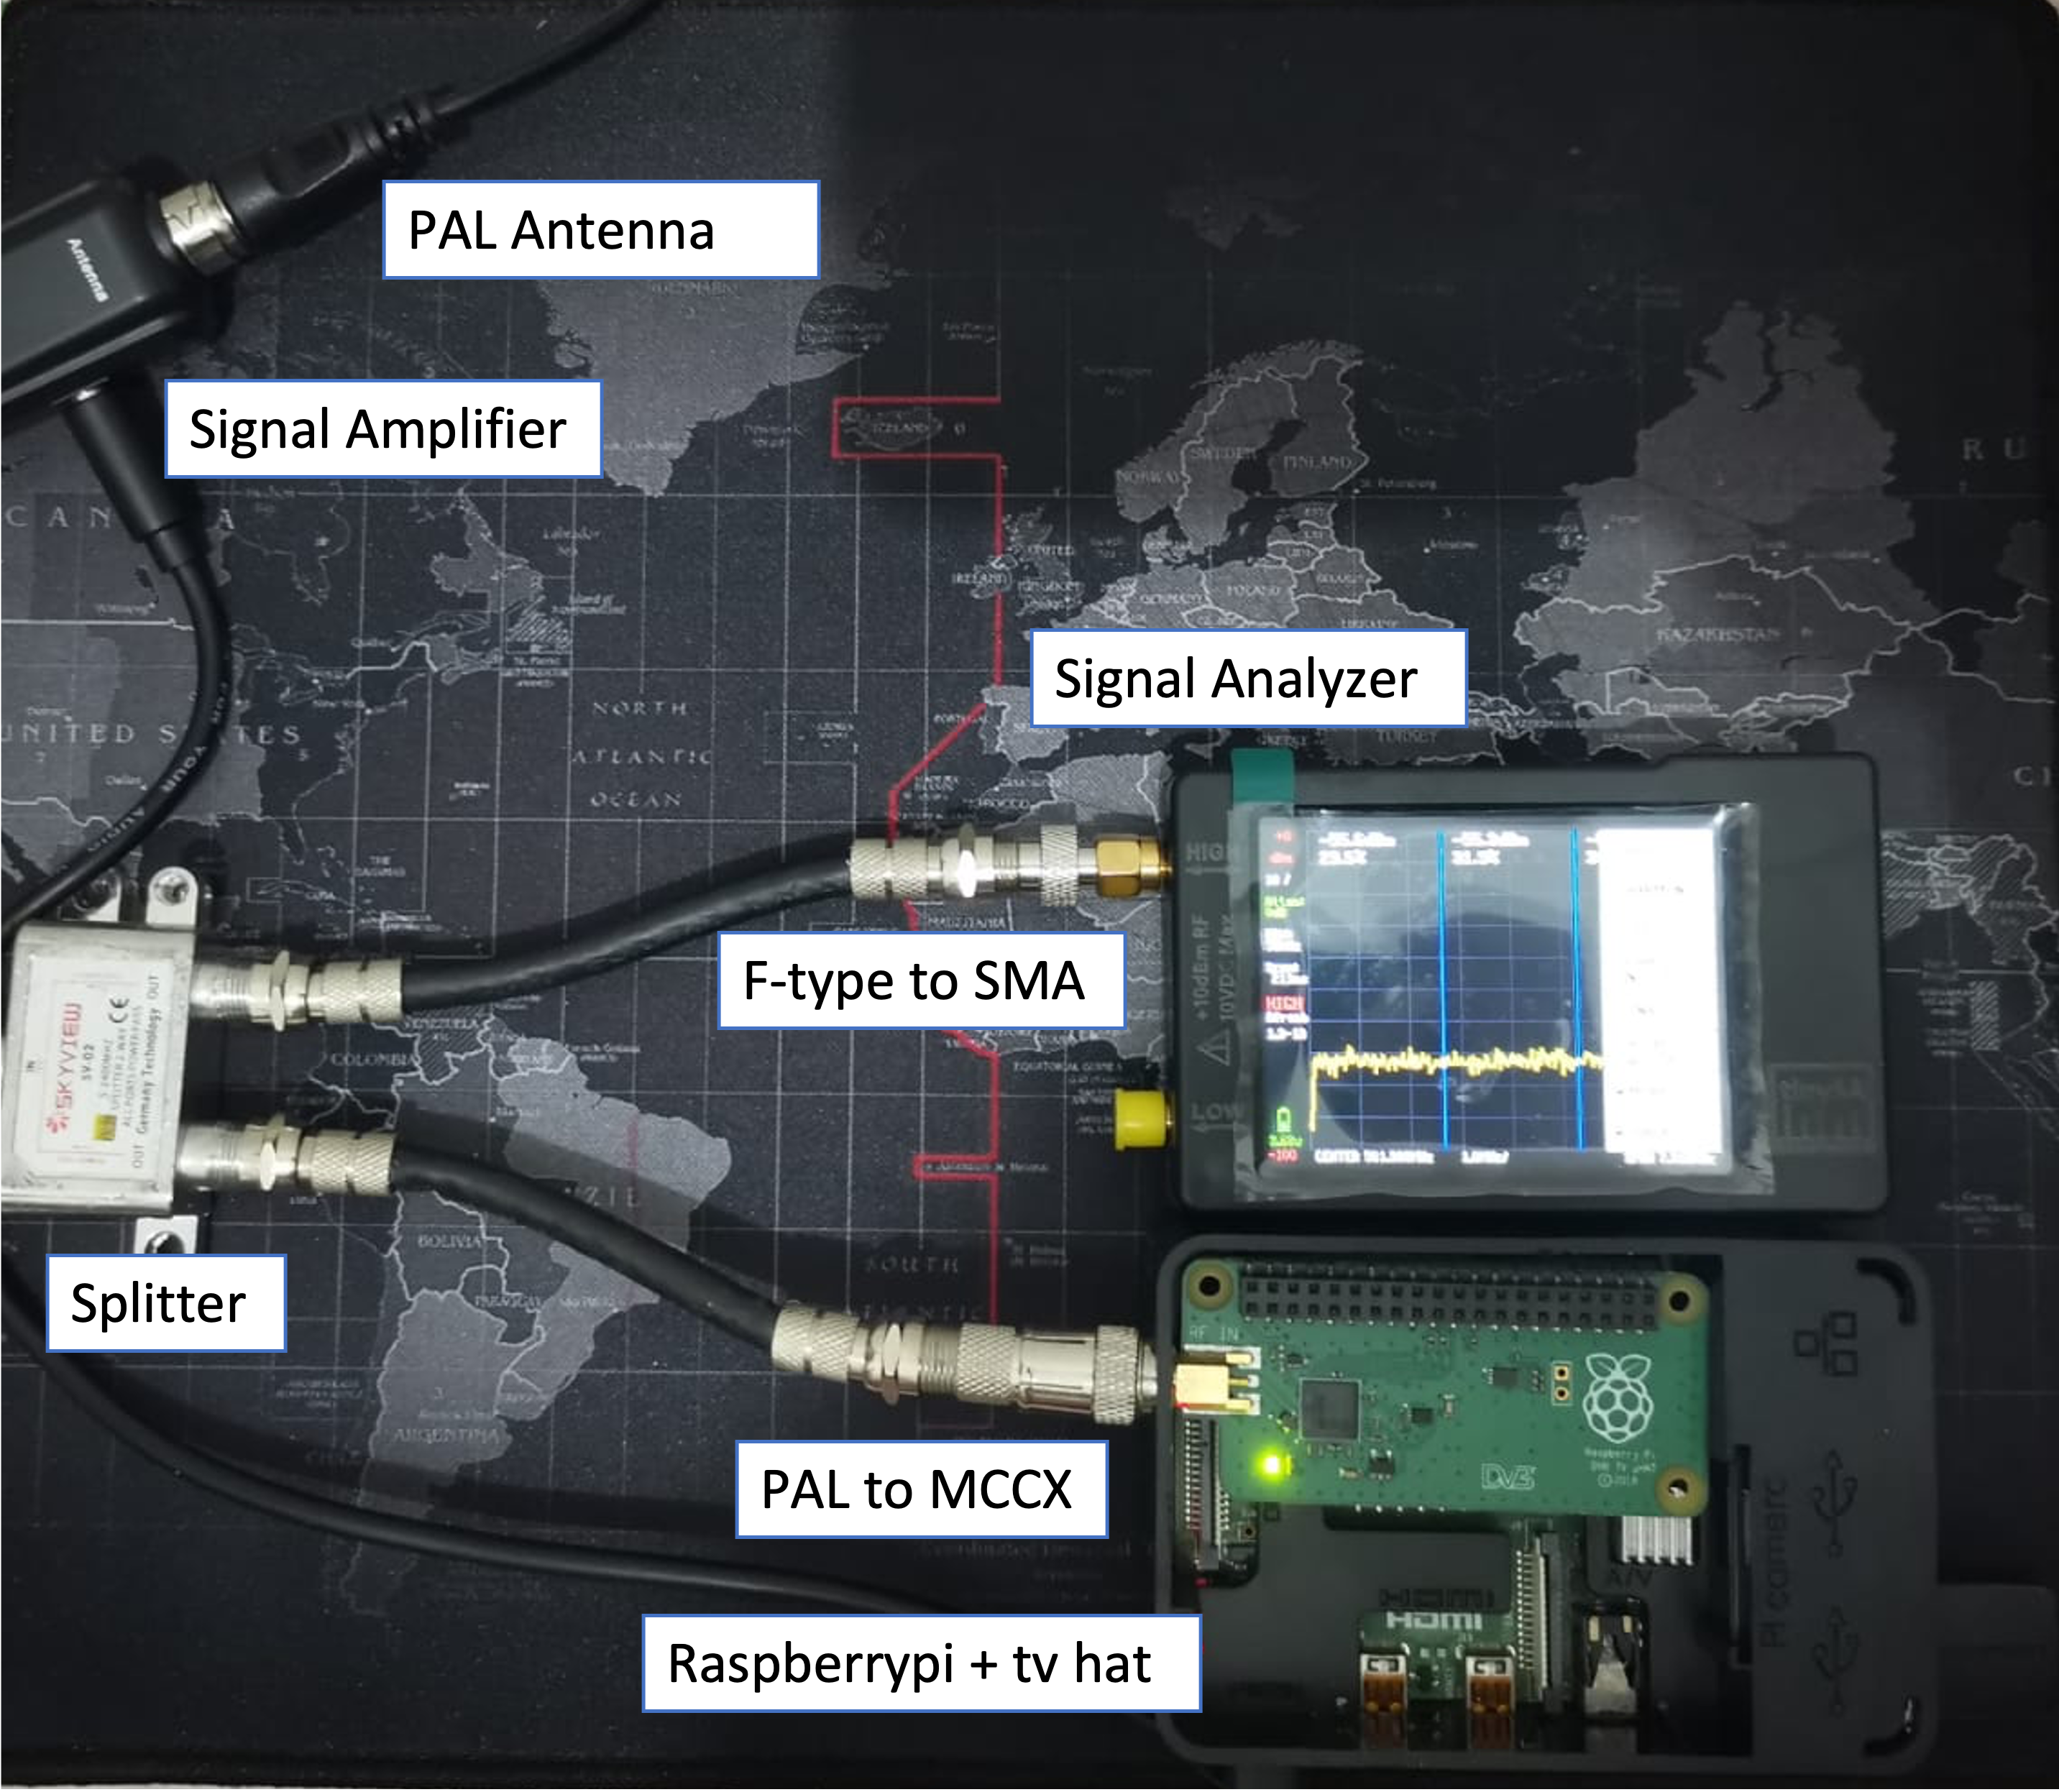
\includegraphics[width=0.9\columnwidth]{bab4/Gambar/hardware-setup.png}
	\end{center}
	\vspace{-0.2cm}
	%\rule{\columnwidth}{0.1pt}
	\caption{Perangkat keras yang digunakan untuk akuisisi video siaran DVB-T2}
	\label{hardware-setup}
\end{figure}
%%%%%%%%%%%%%%%%%%%%%%%%%% GAMBAR %%%%%%%%%%%%%%%%%%%%%%%%%%%%%%

Langkah kedua, memastikan kekuatan sinyal siaran DVB-T2 yang diterima oleh perangkat ada di antara -60 dB sampai -75 dB. Kekuatan sinyal dapat diperkuat menggunakan alat penguat sinyal dan mengubah posisi antena. Kekuatan sinyal dapat diukur menggunakan \textit{tv hat} dengan aplikasi \textit{tvheadend} atau bisa juga menggunakan perangkat signal analyzer seperti yang ditunjukkan pada gambar \ref{tiny-sa}. Ketiga membuat rencana perekaman video menggunakan fitur \textit{record} pada aplikasi \textit{tvheadend}. Perekaman dilakukan dengan beberapa skema untuk memperoleh video dengan kualitas yang baik dan juga video dengan kualitas yang buruk. 

%%%%%%%%%%%%%%%%%%%%%%%%%% GAMBAR %%%%%%%%%%%%%%%%%%%%%%%%%%%%%%
\begin{figure}[H]
	\vspace{-0.1cm}
	%\rule{\columnwidth}{0.1pt}
	\begin{center}
		\includegraphics[width=0.6\columnwidth]{bab4/Gambar/tiny-sa.png}
	\end{center}
	\vspace{-0.2cm}
	%\rule{\columnwidth}{0.1pt}
	\caption{Pengukuran kekuatan sinyal menggunakan \textit{signal analyzer, TinySA}}
	\label{tiny-sa}
\end{figure}
%%%%%%%%%%%%%%%%%%%%%%%%%% GAMBAR %%%%%%%%%%%%%%%%%%%%%%%%%%%%%%

Antena diletakkan diluar bangunan \textit{(outdoor)} dengan ketinggian 2 meter diatas bangunan. Antena yang digunakan adalah antena televisi dengan tipe PX HDA-5000 seperti yang ditunjukkan pada gambar \ref{antenna-5000}. Kemudian dilakukah beberapa skema dengan mengubah posisi antena ke empat arah yang berbeda  selama pengambilan data video. Posisi antena awal $0^\circ$  posisi menghadap ke stasiun pemancar, serta diputar $90^\circ$, $180^\circ$, dan $270^\circ$. Hal ini dilakukan agar mendapatkan gambar dengan kualitas yang bervariasi untuk melengkapi \textit{dataset} yang dibutuhkan.

%%%%%%%%%%%%%%%%%%%%%%%%%% GAMBAR %%%%%%%%%%%%%%%%%%%%%%%%%%%%%%
\begin{figure}[H]
	\vspace{-0.1cm}
	%\rule{\columnwidth}{0.1pt}
	\begin{center}
		\includegraphics[width=0.6\columnwidth]{bab4/Gambar/antenna-5000.png}
	\end{center}
	\vspace{-0.2cm}
	%\rule{\columnwidth}{0.1pt}
	\caption{Penempatan antena outdoor PX HDA-5000}
	\label{antenna-5000}
\end{figure}
%%%%%%%%%%%%%%%%%%%%%%%%%% GAMBAR %%%%%%%%%%%%%%%%%%%%%%%%%%%%%%

Setelah seluruh perangkat sudah siap, maka pengambil data video dapat dilakukan menggunakan aplikasi \textit{tvheadend}. Sebelum menjalankan \textit{tvheadend} pastikan juga sudah melakukan instalasi pada perangkat keras, serta instalasi aplikasi \textit{tvheadend} yang disertai proses pencarian layanan siaran DVB-T2. Selanjutnya dilakukan beberapa konfigurasi pada \textit{tvheadend} dengan malakukan proses perekaman dengan durasi 10 detik per video, dengan interval waktu tertentu. Perekaman dapat menggunakan fitur "\textit{digital video recorder}", kemudian klik  "\textit{upcoming/current recording}", lalu tekan tombol "+" untuk menambahkan jadwal perekaman video seperti yang ditunjukkan pada gambar \ref{tvheadend-record}. Jendela \textit{pop-u}p akan muncul untuk mengisikan judul/nama rekaman, channel/layanan yang dipilih, serta waktu melakukan perekaman. Setelah itu tekan "\textit{apply}". Hasil dari rekaman dapat di download pada tab \textit{"finished recordings"}

%%%%%%%%%%%%%%%%%%%%%%%%%% GAMBAR %%%%%%%%%%%%%%%%%%%%%%%%%%%%%%
\begin{figure}[H]
	\vspace{-0.1cm}
	%\rule{\columnwidth}{0.1pt}
	\begin{center}
		\includegraphics[width=1\columnwidth]{bab4/Gambar/tvheadend-record.png}
	\end{center}
	\vspace{-0.2cm}
	%\rule{\columnwidth}{0.1pt}
	\caption{Fitur melakukan perekaman video siaran DVB-T2 menggunakan \textit{tvheadend}}
	\label{tvheadend-record}
\end{figure}
%%%%%%%%%%%%%%%%%%%%%%%%%% GAMBAR %%%%%%%%%%%%%%%%%%%%%%%%%%%%%%

Selain menggunakan fitur yang terdapat pada \textit{tvheadend} pengambilan video juga dapat dilakukan menggunakan \textit{ffmpeg} dan \textit{python}, namun tetap membutuhkan alamat lokal layanan dari \textit{tvheadend}. Alamat layanan dapat diperoleh dari channel layanan yang terdapat dari tvheadend dan dapat di download dengan format .m3u\textit{ (Moving Picture Experts Group Audio Layer 3 Uniform Resource Locator)}. Digunakan beberapa \textit{library} untuk dapat menjalankan ffmpeg dalam melakukan perekaman dengan interval waktu tertentu. Library yang digunakan adalah \textit{time}, \textit{schedule}, dan \textit{subproses}. Contoh program yang digunakan adalah sebagai berikut:

%%%%%%%%%%%%%%%%%%%%%%%%%% PYTHON %%%%%%%%%%%%%%%%%%%%%%%%%%%%%%
\vspace{0.5cm}	
\begin{lstlisting}[basicstyle=\linespread{0.8}\selectfont, language=Python, numbers=none]
import schedule
import time
import subprocess

def my_function():
	command = 'perintah ffmpeg record + timestamp'
	subprocess.call(shlex.split(command))

schedule.every(1).hours.do(my_function)
while true:
	schedule.run_pending()
	time.sleep(1)
\end{lstlisting}
%%%%%%%%%%%%%%%%%%%%%%%%%% PYTHON %%%%%%%%%%%%%%%%%%%%%%%%%%%%%%

Perekaman materi uji dilakukan dengan durasi 10 detik per video tayangan. Materi video direkam dari lima layanan televisi yang diperoleh di wilayah kota  Depok, Jawa Barat. Layanan televisi yang digunakan sebagai \textit{dataset} adalah TVRI World, TVRI Sport, Metro TV HD, Net TV, dan My TV dengan tiga frekuensi pembawa berbeda . Sudut antena diatur sehingga mendapat kekuatan sinyalyang bervariasi agar mendapatkan hasil data yang dapat menggambarkan kondisi siaran real. Terdapat tiga frekunsi pembawa yang berbeda dari kelima layanan tv tersebut yang ditunjukkan pada tabel \ref{skema-pengukuran}. Lokasi dari ketiga stasiun pemancarnya juga dicatat sebagai penghitungan variabel jarak antara pengirim dan penerima siaran. Jarak line of sight (LOS) antara ketiga stasiun pemancara terhadap perangkat yang digunakan pada penelitan relatif, dimana lokasi pengambilan video dari siaran dilakukan dari kampus F8 Universitas Gunadarma.

%%%%%%%%%%%%%%%%%%%%%%%%%% TABLE %%%%%%%%%%%%%%%%%%%%%%%%%%%%%%
\begin{table}[H]
	\centering
	\setstretch{1.5}
	\caption{Pengambilan \textit{dataset} dari layanan siaran DVB-T2 pada area studi}
	\label{skema-pengukuran}
	\begin{tabular}{|l|l|l|l|l|}
		\hline
		\begin{tabular}[c]{@{}l@{}}Frekuensi \\ Pembawa\end{tabular} & \begin{tabular}[c]{@{}l@{}}Nama \\ Layanan\end{tabular}         & \begin{tabular}[c]{@{}l@{}}Lokasi \\ Pemancar\end{tabular}           & \begin{tabular}[c]{@{}l@{}}Latitude, \\ Langitude\end{tabular} & \begin{tabular}[c]{@{}l@{}}Kekuatan sinyal di\\ $0^\circ$, $90^\circ$, \\ $180^\circ$, $270^\circ$\\ dari pemancar\end{tabular} \\ \hline
		626 MHz                                                      & \begin{tabular}[c]{@{}l@{}}TVRI World\\ TVRI Sport\end{tabular} & \begin{tabular}[c]{@{}l@{}}Tanah Abang,\\ Jakarta Pusat\end{tabular} & \begin{tabular}[c]{@{}l@{}}-6.21254, \\ 106.80071\end{tabular} & \begin{tabular}[c]{@{}l@{}}-64 dBm, -74 dBm\\ -81 dBm, -75 dBm\end{tabular}                                                        \\ \hline
		562 MHz                                                      & \begin{tabular}[c]{@{}l@{}}Metro TV\\ My TV\end{tabular}     & \begin{tabular}[c]{@{}l@{}}Kebon Jeruk,\\ Jakarta Barat\end{tabular} & \begin{tabular}[c]{@{}l@{}}-6.18698,\\ 106.75871\end{tabular}  & \begin{tabular}[c]{@{}l@{}}-64 dBm, -75 dBm\\ -80 dBm, -75 dBm\end{tabular}                                                        \\ \hline
		650 MHz                                                      & Net TV                                                          & \begin{tabular}[c]{@{}l@{}}Kembangan,\\ Jakarta Barat\end{tabular}   & \begin{tabular}[c]{@{}l@{}}-6.22192,\\ 106.71896\end{tabular}  & \begin{tabular}[c]{@{}l@{}}-65 dBm, -75 dBm\\ -81 dBm, -74 dBm\end{tabular}                                                        \\ \hline
		 & \begin{tabular}[c]{@{}l@{}}F8 Universitas\\ Gunadarma\end{tabular} & \begin{tabular}[c]{@{}l@{}}Cimanggis,\\ Kota Depok\end{tabular}      & \begin{tabular}[c]{@{}l@{}}-6.36390,\\ 106.84019\end{tabular}  & Penerima siaran                                                                                                                    \\ \hline	
\end{tabular}
\end{table}
%%%%%%%%%%%%%%%%%%%%%%%%%% TABLE %%%%%%%%%%%%%%%%%%%%%%%%%%%%%%


%%%%%%%%%%%%%%%%%%%%%%%%%% GAMBAR %%%%%%%%%%%%%%%%%%%%%%%%%%%%%%
\begin{figure}[H]
	\vspace{-0.1cm}
	%\rule{\columnwidth}{0.1pt}
	\begin{center}
		\includegraphics[width=1\columnwidth]{bab4/Gambar/jarak-pemancar.png}
	\end{center}
	\vspace{-0.2cm}
	%\rule{\columnwidth}{0.1pt}
	\caption{Jarak stasiun pemancar terhadap lokasi pengambilan data siaran DVB-T2}
	\label{jarak-pemancar}
\end{figure}
%%%%%%%%%%%%%%%%%%%%%%%%%% GAMBAR %%%%%%%%%%%%%%%%%%%%%%%%%%%%%%

Stasiun pemancar terjauh adalah metro tv dengan jarak 22 km. Stasiun siaran TVRI yang berlokasi di kec. Tanah Abang memiliki jarak 18 km, sedangkan yang terdekat adalah stasiun net tv denagn jarak 16 km. Semua pengukuran jarak tersebut diukur secara LOS mengguakan google maps seperti yang ditunjukkan pada gambar \ref{jarak-pemancar}.






\subsection{Koleksi data}
\hspace{1,2cm}
Pengumpulan data merupakan proses terstruktur untuk menghimpun informasi dari berbagai sumber guna mendapatkan wawasan, menganalisis situasi, atau membantu pengambilan keputusan. Melibatkan tahapan perencanaan, identifikasi sumber, pemilihan metode pengumpulan data yang tepat, dan pengolahan data untuk analisis lebih lanjut. Tahapan ini merupakan komponen penting dalam penelitian, uji coba, evaluasi, dan beragam disiplin ilmu lainnya untuk mendukung hipotesis, menguji teori, atau memvalidasi hasil \citep{Yin}.

%%%%%%%%%%%%%%%%%%%%%%%%%% GAMBAR %%%%%%%%%%%%%%%%%%%%%%%%%%%%%%
\begin{figure}[H]
	\vspace{-0.1cm}
	%\rule{\columnwidth}{0.1pt}
	\begin{center}
		\includegraphics[width=1\columnwidth]{bab4/Gambar/hires-img.png}
	\end{center}
	\vspace{-0.2cm}
	%\rule{\columnwidth}{0.1pt}
	\caption{Citra/frame video dengan resolusi FHD $1920\times1080$ piksel hasil rekaman dari siaran DVB-T2}
	\label{hires-img}
\end{figure}
%%%%%%%%%%%%%%%%%%%%%%%%%% GAMBAR %%%%%%%%%%%%%%%%%%%%%%%%%%%%%%

Data yang sudah terkumpul dari hasil akuisisi berupa video dengan durasi 10 detik. Ukuran dari video sekitar 2 MB sampai 10 MB. Gambar \ref{hires-img} merupakan contoh frame yang didapat dari hasil pengambilan video menggunakan prosedur sebelumnya. Diperoleh data dari masing-masing siaran sejumlah 100 video, sehingga terdapat 500 video. Video yang akan dijadikan dataset untuk pengujian obyektif dan subyektif dipilih secara manual dari video yang ada. Pemilihan manual video untuk dataset tersebut berdasarkan kualitas dari video, dari jumlah artefak bloking, bluring dan juga pembekuan frame. Dipilih sejumlah 105 video yang  dijadikan \textit{dataset}. Jumlah dataset awal yang digunakan tidak terlalu besar karena dataset tersebut juga digunakan untuk pengukuran subyektif yang dinilai oleh panelis.

\subsection{Perangkat pengolahan data}
\hspace{1,2cm}
Setelah dipilih sebanyak 105 video untuk \textit{dataset}, maka video akan diukur menggunakan beberapa metrik obyektif spatial dan juga temporal. Pengukuran dilakukan menggunakan dua perangkat komputer untuk pembanding yaitu vm milik \textit{google-colab} dan juga vm \textit{dgx-a100} milik UG. Perangkat tersebut juga digunakan untuk pembuatan model NN dari hasil pengukuran obyektif dan subyektif dari dataset. Spesifikasi umum perangkat yanmg digunakan untuk pengolahan data ditunjukkan pada tabel \ref{nvidia-used}

%%%%%%%%%%%%%%%%%%%%%%%%%% TABLE %%%%%%%%%%%%%%%%%%%%%%%%%%%%%%
\begin{table}[H]
	\centering
	\caption{Perangkat pengolahan data yang digunakan}
	\label{nvidia-used}
	\begin{tabular}{|l|l|}
		\hline
		\rowcolor[HTML]{C0C0C0} 
		\multicolumn{1}{|c|}{\cellcolor[HTML]{C0C0C0}\textbf{Mesin GPU NVIDIA}} & \multicolumn{1}{c|}{\cellcolor[HTML]{C0C0C0}\textbf{Keterangan}} \\ \hline
		Google Colab                                                            & TU104-895-16GB (Tesla 4)                                         \\ \hline
		Universitas Gunadarma                                     & A-100-SXM4-40GB (DGX A00)                                  \\ \hline
	\end{tabular}
\end{table}
%%%%%%%%%%%%%%%%%%%%%%%%%% TABLE %%%%%%%%%%%%%%%%%%%%%%%%%%%%%%


\section{Pengujian metrik obyektif}
\hspace{1,2cm}
Proses pengukuran kualitas video secara obyektif, digunakan tiga metrik. Algoritma metrik obyektif spatial yang digunakan terdiri metrik \textit{blocking} dan metrik \textit{blur}, untuk temporal menggunakan metrik \textit{temporal freeze}. Metrik tersebut  diubah ke dalam bahasa pemprogaman \textit{python} yang kemudian dilakukan pengujian ke beberapa citra/video. Metrik tersebut juga akan digunakan sebagai parameter masukan pada jaringan saraf buatan (NN).

\subsection{Pengujian metrik \textit{blocking}}
\hspace{1,2cm}
Tahap awal mengubah algoritma metrik \textit{blocking} ke dalam bahasa pemprograman python. Kemudian dilakukan pengujian metrik tersebut untuk beberapa citra, dimana semakin besar kerusakannya maka nilainya akan semakin kecil. Interval pengukuran dari metrik ini yaitu $1-100$ dengan skor 1 citra dengan tingkat noise bloking yang tinggi, dan skor 100 citra tanpa bloking. Pseudocode  \ref{metrik-blok} menuliskan secara umum perhitungan yang dilakukan algoritma blok milik Zhou Wang.

%%%%%%%%%%%%%%%%%%% ALGORITMA DAN PESUDO-CODE %%%%%%%%%%%%%%%%%%%%
\begin{algorithm}
	\caption{Metrik pengukuran blok}
	\label{metrik-blok}
	\begin{flushleft}
		\textbf{INPUT:} \textbf{citra}\\
		\textbf{OUTPUT:}	\textbf{blok\_score}
	\end{flushleft}
	\begin{algorithmic}[1]
		\Function{blok\_metric}{$image\_path$}
		\State $img \gets load\_image(image\_path)$ \Comment{Load citra}
		\State $dh \gets img[:, 1:] - img[:, :-1]$ \Comment{Selisih horizontal}
		\State $dv \gets img[1:, :] - img[:-1, :]$ \Comment{Selisih vertikal}
		\State $B_h, B_v \gets \text{Hitung nilai }B_h, B_v$ \Comment{Mean bloking 8x8}
		\State $A_h, A_v \gets \text{Hitung nilai }A_h, A_v$\Comment{Mean dari mean blok - $B_h$}
		\State $sig_h, sig_v \gets \text{Hitung nilai }sig_h, sig_v$ \Comment{Zero crossing}
		\State $Z_h, Z_v \gets \text{Hitung nilai }Z_h, Z_v$ \Comment{Mean zero crossing}
		\State $B, A, Z \gets \text{Hitung nilai }B, A, Z$ \Comment{Mean variabel v dan h}
		\State $score \gets \text{Hitung nilai }score$ \Comment{Skor akhir}
		\State \Return $score$
		\EndFunction
	\end{algorithmic}
\end{algorithm}
%%%%%%%%%%%%%%%%%%% ALGORITMA DAN PESUDO-CODE %%%%%%%%%%%%%%%%%%%%

 Pada gambar \ref{blok-score} dicontohkan nilai luaran yang dihasilkan dari pengukuran metrik \textit{bloking}. Citra yang dicontohkan merupakan hasil cuplikan frame dari video yang ada di dataset.


%%%%%%%%%%%%%%%%%%%%%%%%%% GAMBAR %%%%%%%%%%%%%%%%%%%%%%%%%%%%%%
\begin{figure}[H]
	\vspace{-0.1cm}
	%\rule{\columnwidth}{0.1pt}
	\begin{center}
		\includegraphics[width=0.8\columnwidth]{bab4/Gambar/blok-score.png}
	\end{center}
	\vspace{-0.2cm}
	%\rule{\columnwidth}{0.1pt}
	\caption{Pengukuran metrik obyektif  blok pada citra normal dan \textit{blocking artifact}}
	\label{blok-score}
\end{figure}
%%%%%%%%%%%%%%%%%%%%%%%%%% GAMBAR %%%%%%%%%%%%%%%%%%%%%%%%%%%%%%

Pada gambar \ref{blok-score} menujukkan pengukuran blok pada citra frame siaran DVB-T2 yang ada di \textit{dataset}. Citra bagian atas merupakan citra asli dari siaran, sedangkan citra pada bagian bawah merupakan citra yang sudah diberikan gangguan. Gangguan yang diberikan berupa noise akibat kerusakan data yang terencode dalam proses transmisi. Ditunjukkan citra dengan gangguan blok memiliki skor lebih rendah (skor = 75) dibanding citra asli yang tidak blur (skor = 85) meskipun tidak terlalu signifikan.


%%%%%%%%%%%%%%%%%%%%%%%%%% GAMBAR %%%%%%%%%%%%%%%%%%%%%%%%%%%%%%
\begin{figure}[H]
	\vspace{-0.1cm}
	%\rule{\columnwidth}{0.1pt}
	\begin{center}
		\includegraphics[width=1\columnwidth]{bab4/Gambar/sample-blok.png}
	\end{center}
	\vspace{-0.2cm}
	%\rule{\columnwidth}{0.1pt}
	\caption{Contoh pengukuran metrik obyektif  blok pada beberapa citra siaran televisi DVB-T2}
	\label{sample-blok}
\end{figure}
%%%%%%%%%%%%%%%%%%%%%%%%%% GAMBAR %%%%%%%%%%%%%%%%%%%%%%%%%%%%%%

Pengukuran metrik blok dilakukan secara langsung terhadap citra dari siaran televisi DVB-T2 memiliki beberapa kendala. Seperti yang terlihat pada gambar \ref{sample-blok}, metrik blok tidak signifikan dalam penurunan skor antara gambar dengan kualitas yang baik dan gambar dengan \textit{blocking artifact}. Metrik \textit{bloking} ini juga hanya dapat mendeteksi adanya bloking secara lokal di dalam citra, dan tidak dapat mendeteksi bloking secara menyeluruh di seluruh citra. Hal ini bisa menjadi kekurangan dalam kasus-kasus tertentu di mana bloking yang terjadi lebih kompleks atau terdistribusi secara luas di seluruh citra. Metrik ini juga hanya berfokus pada jenis distorsi \textit{bloking} dan tidak mempertimbangkan distorsi lainnya, seperti distorsi \textit{blur}, \textit{noise}, dan \textit{masking}, sehingga perlu juga dilakukan pengukuran dengan metrik lain.


\subsection{Pengujian metrik \textit{blur}}
\hspace{1,2cm}
Metrik blur pada dasarnya mengukur tingkat kekaburan atau ketidakjelasan pada gambar dengan membandingkan nilai piksel pada tepi gambar dengan nilai piksel sekitarnya. Pengukuran dilakukan dengan cara menghitung perbedaan nilai antara setiap piksel pada tepi gambar dengan nilai piksel terdekat di sekitarnya. Metrik blur menggunakan deteksi tepi pada gambar dengan menggunakan filter Sobel dan menghitung nilai lokal maksimum dan lokal minimum pada tiap tepi gambar. Dalam proses pengukuran, semakin tinggi nilai perbedaan pada tepi gambar dengan nilai piksel di sekitarnya, maka semakin tinggi pula tingkat kekaburan pada citra.

Selanjutnya berdasarkan beberapa percobaan pengukuran pada gambar, hasil dari metrik blur dinormalisasi pada rentang skala 1 hingga 100. Nilai skor 100 menandakan bahwa gambar tidak mengalami kekaburan sedangkan nilai skor 1 menunjukkan bahwa gambar memiliki tingkat kekaburan yang sangat tinggi . Pengukuran yang dilakukan oleh metrik blur dapat membantu dalam mengukur tingkat kekaburan pada gambar yang mungkin sulit diukur secara subjektif oleh manusia, sehingga dapat digunakan sebagai alat bantu dalam memperbaiki atau meningkatkan kualitas gambar. Pada penelitian ini metrik blur dibuat ke bahasa pemprograman \textit{python} untuk melakukan proses pengukuran.


%%%%%%%%%%%%%%%%%%% ALGORITMA DAN PESUDO-CODE %%%%%%%%%%%%%%%%%%%%
\begin{algorithm}
\caption{Metrik pengukuran blur}
\label{metrik-blur}
	\begin{flushleft}
	\textbf{INPUT:} \textbf{citra}\\
	\textbf{OUTPUT:}	\textbf{blur\_score}
		\end{flushleft}
	
		\begin{algorithmic}[1]
		\Function{blur\_metric}{$image\_path$}
		\State $img \gets load\_image(image\_path)$ \Comment{Load citra}
		\State $grayImg \gets convert\_to\_grayscale(img)$ \Comment{Skala abu}
		\State $edgeImg \gets apply\_sobel\_filter(img)$ \Comment{Sobel filter}
		\State $maxVals \gets dilate\_edges(edgeImg)$ \Comment{Lokal maksimum}
		\State $minVals \gets erode\_edges(edgeImg)$ \Comment{Lokal minimum}
		\State $diffImg \gets diff(maxVals, minVals)$ \Comment{Hitung lebar tepi}
		\State $blurMetric \gets sum\_(diffImg)$ \Comment{Jumlah lebar tepi}
		\State $totalEdges \gets count\_edges(edgeImg)$ \Comment{Jumlah seluruh tepi}
		\State $score \gets score(blurMetric, totalEdges)$ \Comment{Menghitung skor}
		\State $score \gets limit\_round\_score(score)$ \Comment{Limit dan bulatkan skor}
		\State \Return $score$
		\EndFunction
	\end{algorithmic}
\end{algorithm}
%%%%%%%%%%%%%%%%%%% ALGORITMA DAN PESUDO-CODE %%%%%%%%%%%%%%%%%%%%

Citra yang sudah disiapkan untuk dialkukan pengujian di unggah ke dalam aplikasi \textit{Jupyter Notebook}. Program juga sudah dituliskan di dalam aplikasi yang sama. Pengukuran pada gambar dilakukan satu persatu dengan urutan proses sepeti yang ditunjukkan pada pseudocode algoritma \ref{metrik-blur}.



%%%%%%%%%%%%%%%%%%%%%%%%%% GAMBAR %%%%%%%%%%%%%%%%%%%%%%%%%%%%%%
\begin{figure}[H]
	\vspace{-0.1cm}
	%\rule{\columnwidth}{0.1pt}
	\begin{center}
		\includegraphics[width=0.8\columnwidth]{bab4/Gambar/blur-score.png}
	\end{center}
	\vspace{-0.2cm}
	%\rule{\columnwidth}{0.1pt}
	\caption{Pengukuran metrik obyektif  blur pada citra normal dan blur}
	\label{blur-score}
\end{figure}
%%%%%%%%%%%%%%%%%%%%%%%%%% GAMBAR %%%%%%%%%%%%%%%%%%%%%%%%%%%%%%

Pada gambar \ref{blur-score} menujukkan pengukuran blur pada citra frame siaran DVB-T2 yang ada di \textit{dataset}. Citra bagian atas merupakan citra asli dari siaran, sedangkan citra pada bagian bawah merupakan citra yang sudah diberikan gangguan \textit{gaussian noise blur} menggunakan library \textit{opencv}. Pada gambar tersebut ditunjukkan citra dengan gangguan blur memiliki skor lebih rendah (skor = 18) dibanding citra asli yang tidak blur (skor = 82).

%%%%%%%%%%%%%%%%%%%%%%%%%% GAMBAR %%%%%%%%%%%%%%%%%%%%%%%%%%%%%%
\begin{figure}[H]
	\vspace{-0.1cm}
	%\rule{\columnwidth}{0.1pt}
	\begin{center}
		\includegraphics[width=1\columnwidth]{bab4/Gambar/sample-blur.png}
	\end{center}
	\vspace{-0.2cm}
	%\rule{\columnwidth}{0.1pt}
	\caption{Contoh pengukuran metrik obyektif  blur pada beberapa citra siaran televisi DVB-T2}
	\label{sample-blur}
\end{figure}
%%%%%%%%%%%%%%%%%%%%%%%%%% GAMBAR %%%%%%%%%%%%%%%%%%%%%%%%%%%%%%

Pengukuran metrik  \textit{blur}  dilakukan secara langsung terhadap citra dari siaran televisi DVB-T2 memiliki beberapa kendala seperti yang terlihat pada gambar \ref{sample-blur}. Metrik blur memiliki ketergantungan pada jenis citra dan kondisi pencahayaan dapat mempengaruhi hasil deteksi tepi dan oleh karena itu dapat mempengaruhi metrik blur. Gambar yang mengalami \textit{bloking} atau \textit{noise} dapat memberikan skor blur yang tinggi karena terdapat banyak tepi baru dari noise \textit{tersebut}, sementara gambar yang gelap dapat memberikan skor blur yang rendah karena tepi yang terlihat samar. Selain itu, pada gambar dengan efek bokeh atau gambar yang dengan sengaja di-\textit{blur}, skor \textit{blur} yang dihasilkan mungkin tidak mencerminkan kualitas \textit{blur} secara objektif.

%%%%%%%%%%%%%%%%%%% ALGORITMA DAN PESUDO-CODE %%%%%%%%%%%%%%%%%%%%
\begin{algorithm}
	\caption{Metrik pengukuran blur}
	\label{metrik-blur}
	\begin{flushleft}
		\textbf{INPUT:} \textbf{citra}\\
		\textbf{OUTPUT:}	\textbf{blur\_score}
	\end{flushleft}
	
	\begin{algorithmic}[1]
		\Function{blur\_metric}{$image\_path$}
		\State $img \gets load\_image(image\_path)$ \Comment{Load citra}
		\State $grayImg \gets convert\_to\_grayscale(img)$ \Comment{Skala abu}
		\State $edgeImg \gets apply\_sobel\_filter(img)$ \Comment{Sobel filter}
		\State $maxVals \gets dilate\_edges(edgeImg)$ \Comment{Lokal maksimum}
		\State $minVals \gets erode\_edges(edgeImg)$ \Comment{Lokal minimum}
		\State $diffImg \gets diff(maxVals, minVals)$ \Comment{Hitung lebar tepi}
		\State $blurMetric \gets sum\_(diffImg)$ \Comment{Jumlah lebar tepi}
		\State $totalEdges \gets count\_edges(edgeImg)$ \Comment{Jumlah seluruh tepi}
		\State $score \gets score(blurMetric, totalEdges)$ \Comment{Menghitung skor}
		\State $score \gets limit\_round\_score(score)$ \Comment{Limit dan bulatkan skor}
		\State \Return $score$
		\EndFunction
	\end{algorithmic}
\end{algorithm}
%%%%%%%%%%%%%%%%%%% ALGORITMA DAN PESUDO-CODE %%%%%%%%%%%%%%%%%%%%

Metrik \textit{blur} juga dapat bergantung pada parameter yang digunakan untuk proses deteksi tepi dan dapat menghasilkan banyak \textit{noise} atau tepi palsu. Oleh karena itu, perlu dilakukan analisis yang lebih komprehensif dan pemilihan metode deteksi tepi yang tepat untuk memperoleh metrik blur yang akurat dan konsisten pada berbagai jenis gambar. Dalam praktiknya, sebaiknya metrik blur digunakan bersama dengan metode pengukuran kualitas gambar lainnya untuk memperoleh hasil yang lebih akurat dan konsisten. Dengan mempertimbangkan faktor-faktor yang dapat mempengaruhi hasil deteksi tepi dan metrik blur, dapat ditemukan teknik-teknik yang lebih canggih dan adaptif untuk pengukuran tingkat blur pada gambar.

\subsection{Pengujian metrik \textit{temporal}}
\hspace{1,2cm}
Pada metrik temporal pengukuran dilakukan terhadap beberapa frame dalam selang waktu tertentu. Metrik ini mengukur tingkat pembekuan \textit{(freeze)} yang terjadi pada frame citra dengan cara menghitung rasio antara jumlah frame membeku terhadap seluruh frame yang diambil. Dalam implementasinya, frame yang dianggap membeku biasanya didefinisikan dengan perubahan piksel yang sangat kecil atau bahkan tidak ada perubahan sama sekali dalam interval waktu tertentu. Hal ini dapat dicapai dengan membandingkan nilai piksel dari dua frame berurutan dan menghitung nilai MSE atau nilai perubahan piksel yang ada. Jika nilai perubahan piksel kurang dari atau sama dengan threshold tertentu, maka frame tersebut dianggap membeku.

%%%%%%%%%%%%%%%%%%%%%%%%%% GAMBAR %%%%%%%%%%%%%%%%%%%%%%%%%%%%%%
\begin{figure}[H]
	\vspace{-0.1cm}
	%\rule{\columnwidth}{0.1pt}
	\begin{center}
		\includegraphics[width=1\columnwidth]{bab4/Gambar/temporal-score.png}
	\end{center}
	\vspace{-0.2cm}
	%\rule{\columnwidth}{0.1pt}
	\caption{Pengukuran metrik temporal \textit{freeze} dengan MSE skor}
	\label{temporal-score}
\end{figure}
%%%%%%%%%%%%%%%%%%%%%%%%%% GAMBAR %%%%%%%%%%%%%%%%%%%%%%%%%%%%%%

Parameter utama yang digunakan pada pengukuran metrik temporal adalah membandingkan dua frame citra saat ini (i) dan sebelumnya (i-1) menggunakan pengukuran \textit{mean square error} (MSE). Nilai maksimal dari MSE bergantung pada ukuran gambar yang digunakan. Semakin besar ukuran gambar, semakin besar nilai maksimal dari MSE. Pada penelitian ini gambar yang digunakan menggunakan ukuran $1920\times1080$ yang artinya nilai maksimal dari MSE nya bisa mencapai $1920\times1080\times3=6220800$ dengan menghitung masing-masing kanal RGB. Sedangkan nilai terkecilnya adalah 0 dengan kondisi kedua citra yang diukur sama persis.  Ditunjukkan  gambar \ref{temporal-score} terdapat empat citra berbeda {A, B, C, D}. Nilai MSE citra A dan B , sedangkan nilai MSE antara citra A dan C adalah besar. Digunakan treshold untuk menetukan apakah gambar mengalami pembekuan dengan nilai MSE kurang dari sama dengan 1, berdasarkan referensi \citep{Quan_Huynh_Thu_2009} dan juga pengujian metrik pada beberapa frame. 

%%%%%%%%%%%%%%%%%%% ALGORITMA DAN PESUDO-CODE %%%%%%%%%%%%%%%%%%%%
\begin{algorithm}
	\caption{Metrik pengukuran blur}
	\label{metrik-temporal}
	\begin{flushleft}
		\textbf{INPUT:} \textbf{video}\\
		\textbf{OUTPUT:}	\textbf{temporal\_score}
	\end{flushleft}
	
	\begin{algorithmic}[1]
		\Function{temporal\_metric}{$image_path_i, image_path_{i-1}$}
		\State $list\_temporal \gets []$
		\For{$i = 1$ to $20$}
		\State $image_i \gets \text{Baca gambar ke-i dari } image\_path_i$
		\State $image_{i-1} \gets \text{Baca gambar ke-(i-1) dari } image\_path_{i-1}$
		\State $mse \gets \text{Hitung nilai MSE antara } image_i \text{ dan } image_{i-1}$
		\If{$mse \leq 1$}
		\State $\text{Tambahkan nilai }1 \text{ ke } list\_temporal$
		\Else
		\State $\text{Tambahkan nilai }0 \text{ ke } list\_temporal$
		\EndIf
		\EndFor
		\State $score \gets  sum(list\_temporal) / len(list\_temporal)$
		\State $score \gets  round(1 - score) * 100$
		\State \Return $score$
		\EndFunction
	\end{algorithmic}
\end{algorithm}
%%%%%%%%%%%%%%%%%%% ALGORITMA DAN PESUDO-CODE %%%%%%%%%%%%%%%%%%%%

Algoritma metrik temporal pembekuan frame ini selanjutnya diterapkan pada video. Dari video dengan durasi 10 detik, diambil 20 frame citra, selanjutnya dilakukan pengukuran terhadap masing-masing citra dibandingkan secara MSE terhadap citra pada frame sebelumnya. Hasilnya akan dicatat kemudian dihitung rata-rata e yang mengalami pembekuan terhadap jumlah seluruh fram yang diambil. Program dituliskan dalam bahasa python seperti yang ditunjukkan pada algoritma pseudocode \ref{metrik-temporal}. Pada algoritma metrik tersbut, semakin besar skornya maka menggambarkan kualitasnya video yang semakin baik dengan interval skor 0-100.

%%%%%%%%%%%%%%%%%%%%%%%%%% GAMBAR %%%%%%%%%%%%%%%%%%%%%%%%%%%%%%
\begin{figure}[H]
	\vspace{-0.1cm}
	%\rule{\columnwidth}{0.1pt}
	\begin{center}
		\includegraphics[width=1\columnwidth]{bab4/Gambar/sample-freeze4.png}
	\end{center}
	\vspace{-0.2cm}
	%\rule{\columnwidth}{0.1pt}
	\caption{Contoh pengukuran metrik obyektif  temporal pada video \textit{dataset} no.84 siaran televisi DVB-T, temporal skor : 90}
	\label{sample-freeze4}
\end{figure}
%%%%%%%%%%%%%%%%%%%%%%%%%% GAMBAR %%%%%%%%%%%%%%%%%%%%%%%%%%%%%%

Pada gambar \ref{sample-freeze4} didapat kemiripan 2 frame dari 20 frame sehingga metrik temporal memberikan skor 90. Sedangkan pada gambar \ref{sample-freeze3} didapat kemiripan frame sebanyak 7 frame, sehingga metrik temporal memberikan skor 65. Semakin banyak frame yang mirip/sama dalam satu video dengan MSE dibawah \textit{treshold} maka akan semakin kecil skor dari metrik temporalnya.

%%%%%%%%%%%%%%%%%%%%%%%%%% TABLE %%%%%%%%%%%%%%%%%%%%%%%%%%%%%%
\begin{table}[H]
	\centering
	\caption{Waktu yang dibutuhkan untuk memproses satu video dalam satuan detik}
	\label{waktu-proses}
	\begin{tabular}{|clcc|c|}
		\hline
		\rowcolor[HTML]{C0C0C0} 
		\multicolumn{1}{|c|}{\cellcolor[HTML]{C0C0C0}\textbf{No.}} &
		\multicolumn{1}{c|}{\cellcolor[HTML]{C0C0C0}\textbf{\begin{tabular}[c]{@{}c@{}}Nama \\ dataset\end{tabular}}} &
		\multicolumn{1}{c|}{\cellcolor[HTML]{C0C0C0}\textbf{\begin{tabular}[c]{@{}c@{}}A\\ Nvidia T4 \\ (Google-colab)\end{tabular}}} &
		\textbf{\begin{tabular}[c]{@{}c@{}}B\\ Nvidia A100\\ (UG)\end{tabular}} &
		\textbf{\begin{tabular}[c]{@{}c@{}}Perbandingan\\ A/B\end{tabular}} \\ \hline
		\multicolumn{1}{|c|}{1} & \multicolumn{1}{l|}{001.mp4} & \multicolumn{1}{c|}{3.8352} & 2.0829 & 1.8413 \\ \hline
		\multicolumn{1}{|c|}{2} & \multicolumn{1}{l|}{007.mp4} & \multicolumn{1}{c|}{3.3550} & 1.7997 & 1.8642 \\ \hline
		\multicolumn{1}{|c|}{3} & \multicolumn{1}{l|}{015.mp4} & \multicolumn{1}{c|}{3.9755} & 2.1446 & 1.8537 \\ \hline
		\multicolumn{1}{|c|}{4} & \multicolumn{1}{l|}{074.mp4} & \multicolumn{1}{c|}{4.8772} & 2.2676 & 2.1508 \\ \hline
		\multicolumn{1}{|c|}{5} & \multicolumn{1}{l|}{084.mp4} & \multicolumn{1}{c|}{4.4204} & 1.9829 & 2.2293 \\ \hline
		\multicolumn{1}{|c|}{6} & \multicolumn{1}{l|}{097.mp4} & \multicolumn{1}{c|}{4.5780} & 1.9934 & 2.2966 \\ \hline
		\multicolumn{1}{|c|}{7} & \multicolumn{1}{l|}{099.mp4} & \multicolumn{1}{c|}{4.6574} & 2.0846 & 2.2342 \\ \hline
		\rowcolor[HTML]{EFEFEF} 
		\multicolumn{4}{|c|}{\cellcolor[HTML]{EFEFEF}Rata-rata}                                       & 2.0671 \\ \hline
	\end{tabular}
\end{table}
%%%%%%%%%%%%%%%%%%%%%%%%%% TABLE %%%%%%%%%%%%%%%%%%%%%%%%%%%%%%

Percobaan dilakukan dengan menggunakan dua mesin GPU untuk mendapat perbedaan waktu proses seperti yang ditunjukkan pada tabel \ref{waktu-proses} Pengujian menggunakan beberapa video untuk menghitung perbandingan skor metrik temporal dengan pengambilan citra sebanyak 20 frame. Dihitung perbandingan antara GPU A yaitu Google colab Nvidia T4 terhadap GPU B milik Universitas Gunadarma NVIDIA A100. Diperoleh waktu proses yang dibutuhkan GPU A 2.0671 kali lebih cepat  dari GPU B.


%%%%%%%%%%%%%%%%%%%%%%%%%% GAMBAR %%%%%%%%%%%%%%%%%%%%%%%%%%%%%%
\begin{figure}[H]
	\vspace{-0.1cm}
	%\rule{\columnwidth}{0.1pt}
	\begin{center}
		\includegraphics[width=1\columnwidth]{bab4/Gambar/sample-freeze3.png}
	\end{center}
	\vspace{-0.2cm}
	%\rule{\columnwidth}{0.1pt}
	\caption{Contoh pengukuran metrik obyektif  temporal pada video \textit{dataset} no.15 siaran televisi DVB-T, temporal skor : 65}
	\label{sample-freeze3}
\end{figure}
%%%%%%%%%%%%%%%%%%%%%%%%%% GAMBAR %%%%%%%%%%%%%%%%%%%%%%%%%%%%%%

Salah satu kekurangan dari metrik temporal freeze adalah kurang mampu menggambarkan kualitas video secara keseluruhan. Metrik ini hanya mampu mendeteksi apakah terjadi freeze pada suatu waktu tertentu dalam video, namun tidak dapat memberikan informasi tentang kualitas video secara keseluruhan atau apakah terdapat jenis distorsi lain seperti blur atau bloking. Selain itu, metrik ini juga dapat memberikan hasil yang tidak akurat jika terdapat frame duplikat, ketidakstabilan dalam pengambilan gambar, atau frame berupa berita yang hanya menampilkan \textit{slide statis}. Oleh karena itu, metrik ini sebaiknya digunakan bersamaan dengan metrik lainnya untuk mendapatkan hasil yang lebih akurat dan lengkap tentang kualitas video. 

\subsection{Pengukuran obyektif pada keseluruhan \textit{dataset}}
\hspace{1.2cm}
Pengukuran obyektif dilakukan pada seluruh dataset yang pada tahapan selanjutnya akan digunakan untuk melakukan pengukuran subyektif. Ketiga metrik obyektif yaitu blok, blur, dan temporal akan diterapkan pada seluruh video untuk memperoleh nilai obyektif dari masing-masing video yang akan digunakan sebagai nilai masukan pada jaringan saraf tiruan NN. Pengukuran dilakukan menggunakan dua super komputer berbeda untuk mendapatkan waktu proses dan kesamaan nilai ukur dari setiap metrik. Pada tabel \ref{obyektif-skor} ditunjukkan sebagian pengukuran yang dilakukan pada dataset. Selanjutnya hasil pengukuran disimpan ke dalam file.csv untuk dilakukan proses selanjutnya ke pengukuran subyektif dan pembuatan model NN.

%%%%%%%%%%%%%%%%%%%%%%%%%% TABLE %%%%%%%%%%%%%%%%%%%%%%%%%%%%%%
\begin{table}[H]
	\centering
	\caption{Pengukuran metrik obyektif terhadap dataset}
	\label{obyektif-skor}
	\begin{tabular}{|l|l|l|l|}
		\hline
		\rowcolor[HTML]{C0C0C0} 
		\textbf{\begin{tabular}[c]{@{}l@{}}Nama \\ video dataset\end{tabular}} &
		\textbf{\begin{tabular}[c]{@{}l@{}}skor \\ metrik blok\end{tabular}} &
		\textbf{\begin{tabular}[c]{@{}l@{}}skor \\ metrik bluk\end{tabular}} &
		\textbf{\begin{tabular}[c]{@{}l@{}}skor \\ metrik temporal\end{tabular}} \\ \hline
		000.mp4 & \multicolumn{1}{c|}{87} & \multicolumn{1}{c|}{39} & \multicolumn{1}{c|}{79}  \\ \hline
		001.mp4 & \multicolumn{1}{c|}{87} & \multicolumn{1}{c|}{79} & \multicolumn{1}{c|}{80}  \\ \hline
		002.mp4 & \multicolumn{1}{c|}{73} & \multicolumn{1}{c|}{20} & \multicolumn{1}{c|}{90}  \\ \hline
		003.mp4 & \multicolumn{1}{c|}{77} & \multicolumn{1}{c|}{49} & \multicolumn{1}{c|}{90}  \\ \hline
		004.mp4 & \multicolumn{1}{c|}{84} & \multicolumn{1}{c|}{80} & \multicolumn{1}{c|}{85}  \\ \hline
		005.mp4 & \multicolumn{1}{c|}{74} & \multicolumn{1}{c|}{50} & \multicolumn{1}{c|}{90}  \\ \hline
		...    & \multicolumn{1}{c|}{...} & \multicolumn{1}{c|}{...} & \multicolumn{1}{c|}{...} \\ \hline
		100.mp4 & \multicolumn{1}{c|}{74} & \multicolumn{1}{c|}{50} & \multicolumn{1}{c|}{90}   \\ \hline
		101.mp4 & \multicolumn{1}{c|}{80} & \multicolumn{1}{c|}{74} & \multicolumn{1}{c|}{85}  \\ \hline
		102.mp4 & \multicolumn{1}{c|}{94} & \multicolumn{1}{c|}{38} & \multicolumn{1}{c|}{100}   \\ \hline
		103.mp4 & \multicolumn{1}{c|}{78} & \multicolumn{1}{c|}{52} & \multicolumn{1}{c|}{85}   \\ \hline
		104.mp4 & \multicolumn{1}{c|}{89} & \multicolumn{1}{c|}{60} & \multicolumn{1}{c|}{75}    \\ \hline
	\end{tabular}
\end{table}
%%%%%%%%%%%%%%%%%%%%%%%%%% TABLE %%%%%%%%%%%%%%%%%%%%%%%%%%%%%%

\section{Hasil pengambilan data pengukuran subyektif}
\hspace{1,2cm}
Pengukuran subjektif kualitas video merupakan langkah penting dalam menilai sejauh mana video memenuhi harapan penonton dan memberikan pengalaman visual yang baik. Proses ini melibatkan penilaian kualitas video berdasarkan persepsi manusia, yang mencakup berbagai faktor seperti kejelasan, kehalusan gerakan, warna, kontras, dan artefak kompresi. Evaluasi kualitas video ini sangat berguna untuk memastikan bahwa video sesuai dengan standar kualitas yang diharapkan oleh penonton dan industri.

Selain itu, pengukuran subjektif juga berperan dalam validasi metrik obyektif yang dikembangkan untuk mengukur kualitas video secara otomatis. Penilaian subjektif digunakan sebagai \textit{ground truth} untuk menguji dan mengoptimalkan metrik obyektif, sehingga mereka dapat lebih akurat dan efektif dalam menggantikan penilaian manusia. Memvalidasi metrik obyektif melalui pengukuran subjektif memungkinkan peneliti dan pengembang untuk menciptakan algoritma penilaian kualitas video yang lebih efisien dan handal.

\subsection{Material pengukuran subyektif}
\hspace{1,2cm}
Pada penelitian ini material yang akan digunakan untuk pengujian adalah dataset berupa video dari siaran DVB-T2 sebanyak 105 video. Pada tahap sebelumnya sudah dilakukan pengukuran menggunakan metrik obyektif spatial dan temporal pada video tersebut. Terdapat tiga metrik obyektif yang sudah diterapkan dan mendapatkan skornya masing-masing untuk seluruh video. Di pengujian kali ini akan dilakukan pengukuran secara subyektif pada video tersebut. Tujuan dari pengukuran subyektif pada kualitas video adalah untuk mendapatkan penilaian kualitas video dari sudut pandang manusia, dengan melibatkan partisipasi pengamat manusia untuk memberikan penilaian secara langsung terhadap video yang ditampilkan.

\subsection{Perangkat yang digunakan}
\hspace{1,2cm}
Perangkat yang digunakan untuk melakukan pengukuran subyektif berupa perangkat keras laptop Macbook Pro 2019 hexa-core i7 RAM DDR4 16GB dan perangkat lunak yang dibuat secara mandiri. Perangkat lunak berupa aplikasi web yang menggunakan \textit{native javascript}, css dan html yang terintall secara lokal pada laptop. Seluruh materi video yang akan diujan dimasukan ke dalam aplikasi. Selanjutnya pengujian akan dilakukan menggunakan laptop tersebut satu persatu olehpanelis/partisipan.

\subsection{Proses pengukuran subyektif }
\hspace{1.2cm}
Pengukuran subyektif atau \textit{(subjective assessment)} yang dilakukan pada penelitian ini menggunakan standar pengukuran ITU-R BT.500-14 tahun 2019 mengenai standarisasi prosedur untuk melakukan subyektif tes pada citra televisi. Pengukuran subyektif melibatkan 25 yang terdiri dari 21 laki-laki dan 4 perempuan.  Kriteria dari panelis yaitu rentang usia 20 - 40 tahun dikarenakan berdasarkan data dari organisasi survei Nielsen diperoleh jumlah penonton televisi terbanyak di Indonesia yaitu 41\% berada pada rentang umur tersebut \citep{Annur2023}. Kriteria lainnya yaitu pernah menonton televisi digital dan tidak memiliki gangguan mata. Selanjutnya masing-masing panelis akan memberikan penilaian terhadap keseluruhan dataaset sebanyak 105 video menggunakan aplikasi yang sudah dibuat.

%%%%%%%%%%%%%%%%%%%%%%%%%% GAMBAR %%%%%%%%%%%%%%%%%%%%%%%%%%%%%%
\begin{figure}[H]
	\vspace{-0.1cm}
	%\rule{\columnwidth}{0.1pt}
	\begin{center}
		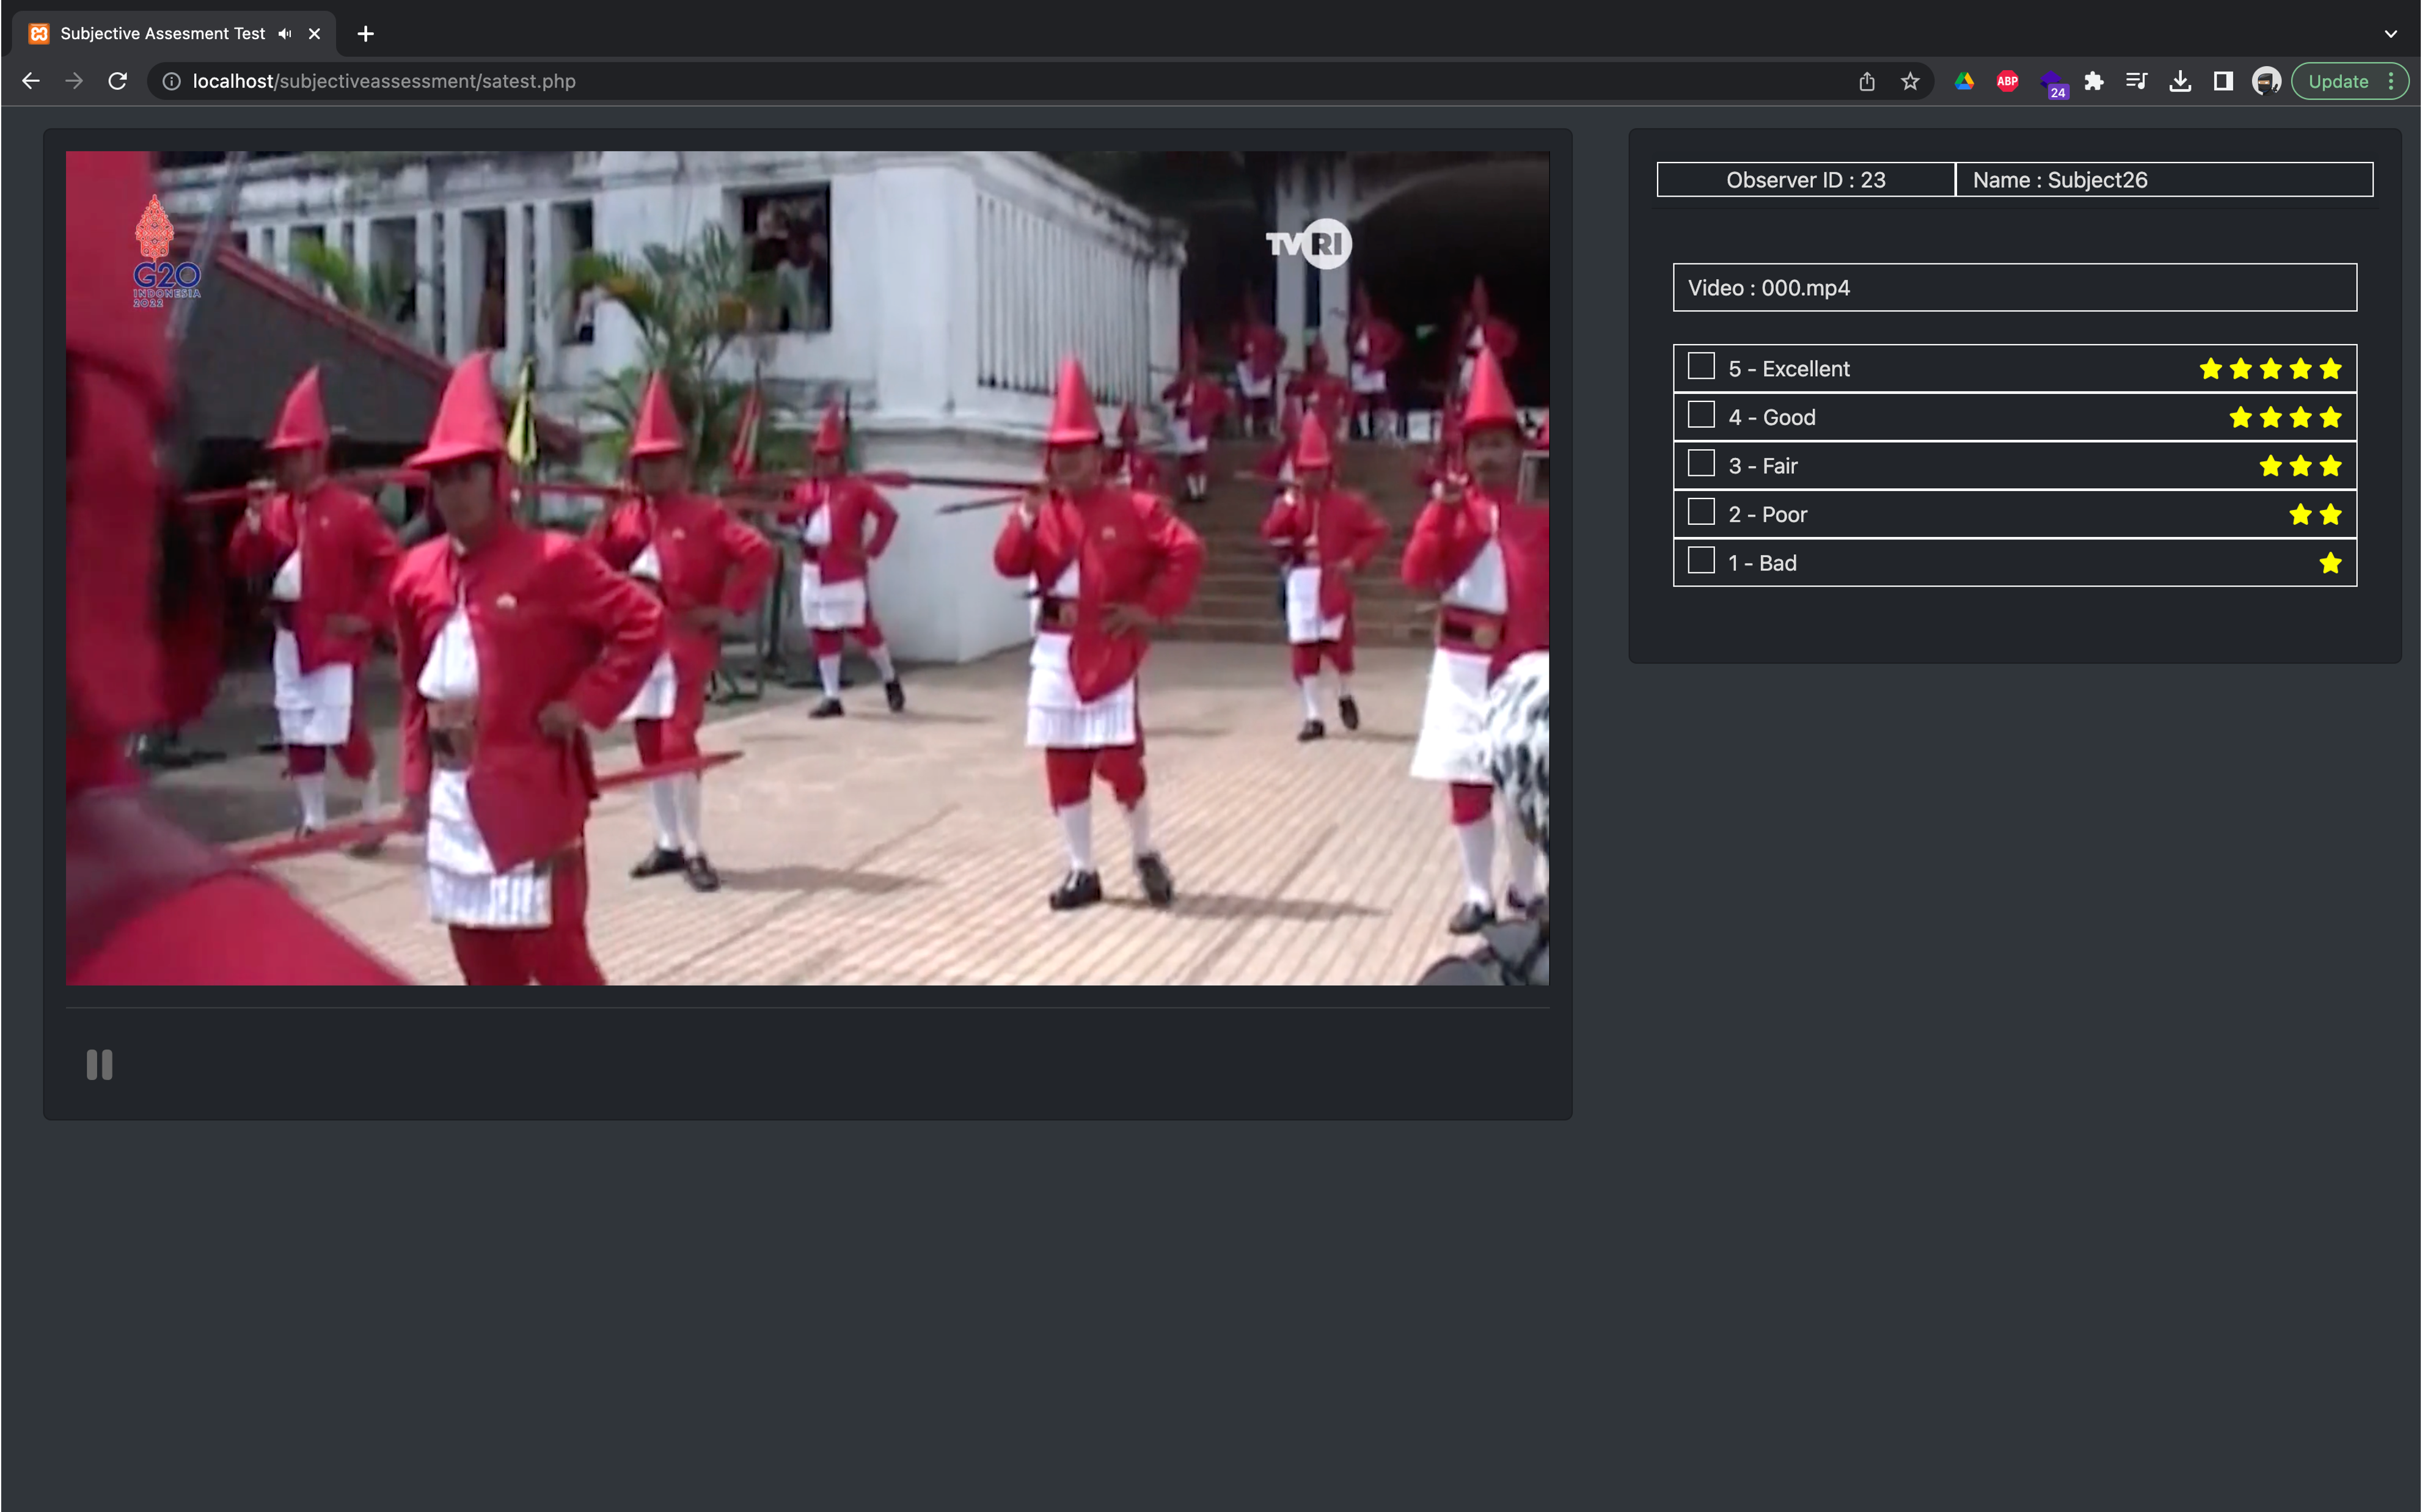
\includegraphics[width=1\columnwidth]{bab4/Gambar/aplikasi-tes.png}
	\end{center}
	\vspace{-0.2cm}
	%\rule{\columnwidth}{0.1pt}
	\caption{Tampilan aplikasi pengukuran subyektif kualitas citra video siaran DVB-T2}
	\label{aplikasi-tes}
\end{figure}
%%%%%%%%%%%%%%%%%%%%%%%%%% GAMBAR %%%%%%%%%%%%%%%%%%%%%%%%%%%%%%

Metode yang digunakan untuk pelakukan pengukuran subyektif pada penelitian ini adalah \textit{single stimulus} (SS). Panelis akan duduk di depan laptop dengan kondisi \textit{home-environment}. Kemudian panelis menjalankan aplikasi tes, melakukan latihan dan pengarahan, selanjutkan masuk kebagian sesi utama tes. Pada tes ini setiap video dengan durasi 10 detik akan diputarkan dengan jeda 4 detik antar videonya. Sehingga untuk menyelesaikan 105 video, panelis membutuhkan waktu sekitar 24.5 menit. Panelis harus memberikan penilaian pada setiap video dengan skor 1 sampai 5. Skor tersebut menggambarkan kualitas video dengan skor 1 artinya sangat buruk dan skor 5 berarti sangat baik dari sisi kualitas citranya. Tampilan dari sesi utama tes ditunjukkan pada gambar \ref{aplikasi-tes}.

%%%%%%%%%%%%%%%%%%%%%%%%%% GAMBAR %%%%%%%%%%%%%%%%%%%%%%%%%%%%%%
\begin{figure}[H]
	\vspace{-0.1cm}
	%\rule{\columnwidth}{0.1pt}
	\begin{center}
		\includegraphics[width=1\columnwidth]{bab4/Gambar/aplikasi-admin.png}
	\end{center}
	\vspace{-0.2cm}
	%\rule{\columnwidth}{0.1pt}
	\caption{Tampilan dashboard aplikasi pengukuran subyektif dari sisi administrator}
	\label{aplikasi-admin}
\end{figure}
%%%%%%%%%%%%%%%%%%%%%%%%%% GAMBAR %%%%%%%%%%%%%%%%%%%%%%%%%%%%%%

Setelah panelis melakukan tes, maka data dapat diakses oleh administrator web  pada bagian dashboard. Ditampilkan jumlah peserta yang sudah memeberikan penilaian dan skor rata-rata per video seperti yang ditunjukkan pada gambar \ref{aplikasi-admin}. Data juga bisa di dowload dengan format .xls untuk selanjutnya diolah. 

\subsection{Hasil pengukuran subyektif}
\hspace{1,2cm}
Setelah data penilaian subjektif terkumpul dari panelis, beberapa langkah pengolahan data perlu dilakukan untuk menghitung hasil pengukuran subjektif dan menganalisis hasil tersebut. Seperti yang ditunjukkan pada tabel \ref{} langkah yang perlu diambil meliputi menghitung nilai rata-rata (Mean Opinion Score/MOS) untuk setiap klip video, menghitung deviasi standar dan interval kepercayaan 95\%.

%%%%%%%%%%%%%%%%%%%%%%%%%% TABLE %%%%%%%%%%%%%%%%%%%%%%%%%%%%%%
\begin{table}[H]
	\fontsize{9pt}{9pt}\selectfont
	\centering
	\caption{Hasil pengukuran subyektif terhadap dataset}
	\label{obyektif-skor}
	% Please add the following required packages to your document preamble:
	% \usepackage[table,xcdraw]{xcolor}
	% If you use beamer only pass "xcolor=table" option, i.e. \documentclass[xcolor=table]{beamer}
		\begin{tabular}{|c|c|c|c|c|c|}
			\hline
			\rowcolor[HTML]{EFEFEF} 
			Nama    & MOS  & Stdev & Conf\_Int & Batas\_bawah & Batas\_atas \\ \hline
			000.mp4 & 3.80 & 0.82  & 0.16      & 3.64         & 3.96        \\ \hline
			001.mp4 & 4.64 & 0.64  & 0.12      & 4.52         & 4.76        \\ \hline
			002.mp4 & 2.24 & 0.88  & 0.17      & 2.07         & 2.41        \\ \hline
			003.mp4 & 1.60 & 0.58  & 0.11      & 1.49         & 1.71        \\ \hline
			004.mp4 & 1.84 & 0.62  & 0.12      & 1.72         & 1.96        \\ \hline
			005.mp4 & 2.04 & 0.89  & 0.17      & 1.87         & 2.21        \\ \hline
			006.mp4 & 1.48 & 0.59  & 0.11      & 1.37         & 1.59        \\ \hline
			007.mp4 & 1.00 & 0.00  & 0.00      & 1.00         & 1.00        \\ \hline
			008.mp4 & 1.64 & 0.64  & 0.12      & 1.52         & 1.76        \\ \hline
			009.mp4 & 3.96 & 0.79  & 0.15      & 3.81         & 4.11        \\ \hline
			010.mp4 & 4.20 & 0.76  & 0.15      & 4.05         & 4.35        \\ \hline
			...     & ...  & ...   & ...       & ...          & ...         \\ \hline
			091.mp4 & 3.56 & 0.71  & 0.14      & 3.42         & 3.70        \\ \hline
			092.mp4 & 2.12 & 0.73  & 0.14      & 1.98         & 2.26        \\ \hline
			093.mp4 & 2.00 & 0.50  & 0.10      & 1.90         & 2.10        \\ \hline
			094.mp4 & 1.60 & 0.71  & 0.14      & 1.46         & 1.74        \\ \hline
			095.mp4 & 1.04 & 0.20  & 0.04      & 1.00         & 1.08        \\ \hline
			096.mp4 & 4.16 & 0.69  & 0.13      & 4.03         & 4.29        \\ \hline
			097.mp4 & 4.68 & 0.56  & 0.11      & 4.57         & 4.79        \\ \hline
			098.mp4 & 4.20 & 0.71  & 0.14      & 4.06         & 4.34        \\ \hline
			099.mp4 & 4.20 & 0.65  & 0.12      & 4.08         & 4.32        \\ \hline
			100.mp4 & 4.68 & 0.56  & 0.11      & 4.57         & 4.79        \\ \hline
			101.mp4 & 2.20 & 0.65  & 0.12      & 2.08         & 2.32        \\ \hline
			102.mp4 & 4.12 & 0.73  & 0.14      & 3.98         & 4.26        \\ \hline
			103.mp4 & 2.32 & 0.85  & 0.16      & 2.16         & 2.48        \\ \hline
			104.mp4 & 4.12 & 0.83  & 0.16      & 3.96         & 4.28        \\ \hline
		\end{tabular}
\end{table}
%%%%%%%%%%%%%%%%%%%%%%%%%% TABLE %%%%%%%%%%%%%%%%%%%%%%%%%%%%%%

Pengukuran dilakukan pada masing-masing video, MOS menunjukkan nilai rata-rata dari seluruh panelis yang melakukan tes. Semakin besar nilai dari MOS menunjukkan semakin bagus kualitas video tersebut. Standar deviasi dari data (Stdev) menunjukkan variasi panelis dalam memberikan nilai, semakin besar stdev-nya, maka semakin bervariasi panelis dalam memberikan penilaian. Dilakukan juga pengukuran interval kepercayaan 95\% untuk memberikan nilai batas bawah dan batas atas rata-rata dari polpulasi sebenarnya. 

%%%%%%%%%%%%%%%%%%%%%%%%%% GAMBAR %%%%%%%%%%%%%%%%%%%%%%%%%%%%%%
\begin{figure}[H]
	\vspace{-0.1cm}
	%\rule{\columnwidth}{0.1pt}
	\begin{center}
		\includegraphics[width=1\columnwidth]{bab4/Gambar/sebaran-tes.png}
	\end{center}
	\vspace{-0.2cm}
	%\rule{\columnwidth}{0.1pt}
	\caption{Sebaran MOS pengukuran tes subyektif dari dataset video}
	\label{sebaran-tes}
\end{figure}
%%%%%%%%%%%%%%%%%%%%%%%%%% GAMBAR %%%%%%%%%%%%%%%%%%%%%%%%%%%%%%

%%%%%%%%%%%%%%%%%%%%%%%%%% GAMBAR %%%%%%%%%%%%%%%%%%%%%%%%%%%%%%
\begin{figure}[H]
	\vspace{-0.1cm}
	%\rule{\columnwidth}{0.1pt}
	\begin{center}
		\includegraphics[width=1\columnwidth]{bab4/Gambar/sort-tes.png}
	\end{center}
	\vspace{-0.2cm}
	%\rule{\columnwidth}{0.1pt}
	\caption{Pembagian kelas MOS pengukuran subyektif dataset }
	\label{sort-tes}
\end{figure}
%%%%%%%%%%%%%%%%%%%%%%%%%% GAMBAR %%%%%%%%%%%%%%%%%%%%%%%%%%%%%%

%%%%%%%%%%%%%%%%%%%%%%%%%% GAMBAR %%%%%%%%%%%%%%%%%%%%%%%%%%%%%%
\begin{figure}[H]
	\vspace{-0.1cm}
	%\rule{\columnwidth}{0.1pt}
	\begin{center}
		\includegraphics[width=1\columnwidth]{bab4/Gambar/var-tes.png}
	\end{center}
	\vspace{-0.2cm}
	%\rule{\columnwidth}{0.1pt}
	\caption{Varian pengukuran subyektif dataset dengan skor terurut}
	\label{var-tes}
\end{figure}
%%%%%%%%%%%%%%%%%%%%%%%%%% GAMBAR %%%%%%%%%%%%%%%%%%%%%%%%%%%%%%

Berdasarkan hasil \textit{scatter plot} dari gambar \ref{sebaran-tes} yang menunjukkan sebaran data dari pengukuran subyektif, diperoleh lebih banyak skor MOS pengukuran terdapat pada rentang 3.5 sampai 4.5. Kemudian data diurutkan dari skor MOS terkecil hingga terbesar seperti yang ditunjukkan pada gambar \ref{sort-tes}. Jika data dipisahkan menjadi 5 kelas berbeda sesuai dengan penilaian pada standar ITU-R BT.500-14 maka diperoleh batasan seperti pada tabel \ref{batas-kelas}. Batasan tersebut yang digunakan sebagai acuan untuk menentukan batasan skor pada pengukuran secara waktu nyata. Selanjutnya dilakukan pengukuran terhadap variansi dari masing-masing data. Seperti yang ditunjukkan pada gambar \ref{var-tes} nilai variansi tertinggi berada pada data urutan ke 40-60. Hal tersebut berarti banyak varian panelis pada rentang tersebut yaitu pada kelas klasifikasi 3.

%%%%%%%%%%%%%%%%%%%%%%%%%% TABLE %%%%%%%%%%%%%%%%%%%%%%%%%%%%%%
\begin{table}[H]
	\fontsize{12pt}{12pt}\selectfont
	\centering
	\caption{Batasan masing-masing kelas berdasarkan pengukuran subyektif}
	\label{batas-kelas}
	% Please add the following required packages to your document preamble:
	% \usepackage[table,xcdraw]{xcolor}
	% If you use beamer only pass "xcolor=table" option, i.e. \documentclass[xcolor=table]{beamer}
	\begin{tabular}{|c|c|c|c|c|}
		\hline
		\rowcolor[HTML]{EFEFEF} 
		Kelas & Jumlah data & Batas bawah & Batas atas & \multicolumn{1}{l|}{\cellcolor[HTML]{EFEFEF}Interval batas} \\ \hline
			1 & 20 & 1.00 & 1.96 & 0.96 \\ \hline
			2 & 20 & 1.96 & 3.20 & 1.06 \\ \hline
			3 & 20 & 3.20 & 4.12 & 0.92 \\ \hline
			4 & 20 & 4.12 & 4.32 & 0.20 \\ \hline
			5 & 20 & 4.32 & 5.00 & 0.68 \\ \hline
	\end{tabular}
\end{table}
%%%%%%%%%%%%%%%%%%%%%%%%%% TABLE %%%%%%%%%%%%%%%%%%%%%%%%%%%%%%

Berdasakan hasil dari pengukuran subyektif kemudian dibagi menjadi 5 kelas dengan jumlah data yang sama. Dikarenakan distribusi yang tidak merata maka interval antar kelas berbeda-beda. Interval tertinggi berada pada kelas 2, dan interval terendah berada pada kelas 4. Selanjutnya data hasil pengukuran subyektif  ini akan digunakan sebagai parameter luaran pada NN.


\section{Pengujian dan hasil pada NN}
\hspace{1,2cm}
Pengujian yang dilakukan dalam membentuk model NN adalah akurasi dan korelasi dari model tersebut. Luaran model NN yang dibentuk yaitu untuk menentukan kualitas suatu video pada siaran DVB-T2. Terdapat 100 dataset yang sudah di label menggunakan hasil pengukuran subyektif. Parameter tersebut berupa luaran dari NN yang akan dibentuk. Terdapat juga tiga parameter masukan pada NN yaitu metrik blok, metrik blur dan metrik temporal freeze. Masukan dan luaran pada NN tersebut buat skor dari metrik dengan obyek video yang sudah diukur, bukan videonya secara langsung. Pengujian dilakukan menggunakan beberapa jenis NN, seperti artificial Neural Netrwok (ANN), atau recurrent neural network (RNN).

\subsection{Data masukan dan luaran model}
\hspace{1,2cm}
Terdapat 100 dataset berupa skor dari pengukuran menggunakan metrik obyektif pada video siaran DVB-T2. Luaran yang ingin dicapai adalah kemiripan dengan MOS hasil pengukuran subyektif yang sudah dilakukan oleh panelis pada 100 video. Pada tabel \ref{overall-skor} ditunjuukan sebagian hasil pengukuran metrik obyektif dan juga skor MOS pada pengukuran subyektif.

\begin{table}[H]
	\fontsize{9pt}{9pt}\selectfont
	\centering
	\caption{Hasil pengukuran subyektif terhadap dataset}
	\label{overall-skor}
	% Please add the following required packages to your document preamble:
	% \usepackage[table,xcdraw]{xcolor}
	% If you use beamer only pass "xcolor=table" option, i.e. \documentclass[xcolor=table]{beamer}
	% Please add the following required packages to your document preamble:
	% \usepackage[table,xcdraw]{xcolor}
	% If you use beamer only pass "xcolor=table" option, i.e. \documentclass[xcolor=table]{beamer}
		\begin{tabular}{|c|c|c|c|c|c|c|c|c|}
			\hline
			\rowcolor[HTML]{EFEFEF} 
			nama    & m\_blok & m\_blur & m\_grad & std\_grad & move\_fr & m\_temp & mos  & class \\ \hline
			000.mp4 & 87      & 52      & 4.84    & 4.76      & 95          & 75          & 3.8  & 3     \\ \hline
			001.mp4 & 88      & 55      & 0.29    & 0.25      & 100         & 75          & 4.64 & 5     \\ \hline
			002.mp4 & 73      & 1       & -0.26   & 0.12      & 50          & 90          & 2.24 & 2     \\ \hline
			003.mp4 & 79      & 8       & 3.85    & 8.5       & 71          & 90          & 1.6  & 1     \\ \hline
			004.mp4 & 80      & 10      & 0.33    & 4.94      & 75          & 85          & 1.84 & 1     \\ \hline
			005.mp4 & 73      & 2       & 3.67    & 8.12      & 71          & 90          & 2.04 & 2     \\ \hline
			006.mp4 & 72      & 42      & -0.51   & 0.59      & 49          & 90          & 1.48 & 1     \\ \hline
			007.mp4 & 48      & 13      & 3.9     & 9.97      & 71          & 35          & 1    & 1     \\ \hline
			008.mp4 & 72      & 10      & -0.35   & 0.63      & 50          & 90          & 1.64 & 1     \\ \hline
			009.mp4 & 86      & 52      & 1.63    & 0.78      & 98          & 80          & 3.96 & 3     \\ \hline
			010.mp4 & 78      & 9       & 0       & 0.31      & 100         & 85          & 4.2  & 4     \\ \hline
			...	 & ...      & ...       & ...      & ...      & ...        & ...          & ...  & ...     \\ \hline
			091.mp4 & 70      & 14      & -0.25   & 0.51      & 50          & 80          & 3.56 & 3     \\ \hline
			092.mp4 & 74      & 12      & 2.21    & 2.6       & 98          & 75          & 2.12 & 2     \\ \hline
			093.mp4 & 67      & 40      & -0.28   & 0.59      & 50          & 80          & 2    & 2     \\ \hline
			094.mp4 & 68      & 50      & -0.23   & 0.38      & 50          & 85          & 1.6  & 1     \\ \hline
			095.mp4 & 76      & 44      & 1.3     & 2.92      & 74          & 65          & 1.04 & 1     \\ \hline
			096.mp4 & 95      & 52      & 4       & 1.57      & 96          & 90          & 4.16 & 4     \\ \hline
			097.mp4 & 80      & 0       & 0.29    & 0.46      & 100         & 90          & 4.68 & 5     \\ \hline
			098.mp4 & 82      & 9       & 0.1     & 0.26      & 100         & 75          & 4.2  & 4     \\ \hline
			099.mp4 & 94      & 70      & 2.68    & 1.82      & 97          & 90          & 4.2  & 4     \\ \hline
			100.mp4 & 87      & 76      & 2.12    & 2.95      & 98          & 90          & 4.68 & 5     \\ \hline
			101.mp4 & 79      & 65      & -0.47   & 0.58      & 50          & 85          & 2.2  & 2     \\ \hline
			102.mp4 & 92      & 52      & 9.33    & 16.3      & 66          & 100         & 4.12 & 4     \\ \hline
			103.mp4 & 78      & 21      & 1.86    & 7.08      & 73          & 85          & 2.32 & 2     \\ \hline
			104.mp4 & 86      & 52      & 1.36    & 2.3       & 99          & 75          & 4.12 & 4     \\ \hline
		\end{tabular}
\end{table}
%%%%%%%%%%%%%%%%%%%%%%%%%% TABLE %%%%%%%%%%%%%%%%%%%%%%%%%%%%%%

%%%%%%%%%%%%%%%%%%%%%%%%%% GAMBAR DUA %%%%%%%%%%%%%%%%%%%%%%%%%%%%%%
\begin{figure}[H]
\vspace{-0.2cm}
\begin{center}
	\begin{tabular}{cc}
		\includegraphics[width=1\columnwidth]{bab4/Gambar/mos-blok.png} \\
		(a) \\
		\includegraphics[width=1\linewidth]{bab4/Gambar/mos-blur.png} \\
		(b) \\  
	\end{tabular}
\end{center}
	\vspace{-0.1cm}
	\caption{Diagram scatter pengukuran metrik spatial terhadap MOS pada pengukuran subyektif (a) metrik blok, (b) metrik blur.}
	\label{metrik-spatial}
\end{figure}
%%%%%%%%%%%%%%%%%%%%%%%%%% GAMBAR DUA %%%%%%%%%%%%%%%%%%%%%%%%%%%%%%

%%%%%%%%%%%%%%%%%%%%%%%%%% GAMBAR DUA %%%%%%%%%%%%%%%%%%%%%%%%%%%%%%
\begin{figure}[H]
	\vspace{-0.2cm}
	\begin{center}
		\begin{tabular}{cc}
			\includegraphics[width=1\linewidth]{bab4/Gambar/mos-temp.png} \\
			(a)  \\
			\includegraphics[width=1\linewidth]{bab4/Gambar/mos-grad.png} \\
			(b) \\
		\end{tabular}
	\end{center}
	\vspace{-0.1cm}
	\caption{Diagram scatter pengukuran metrik temporal terhadap MOS pada pengukuran subyektif (a) metrik freeze, (b) metrik variansi gradien .}
	\label{metrik-temp}
\end{figure}
%%%%%%%%%%%%%%%%%%%%%%%%%% GAMBAR DUA %%%%%%%%%%%%%%%%%%%%%%%%%%%%%%
\newpage


\subsection{Pengujian arsitektur NN}
\hspace{1,2cm}
Pengujian untuk mencari arsitektur NN yang sesuai dengan menggunakan tiga metode. Metode pertama adalah dengan menggunakan regresi multivariable, kedua menggunakan ANN tanpa klasifikasi kelas, yang ketiga dengan menggunakan ANN dan RNN dengan klasifikasi. Ketiga metode tersebut dilakukan untuk mencari tingkat akurasi dan korelasi paling tinggi, serta waktu paling cepat dalam menentukan nilai dari data baru.

\subsubsection{Hasil regresi multivariabel}
\hspace{1,2cm}
Regresi multivariabel digunakan untuk mencari bobot dari setiap variabel masukan yang digunakan untuk menentukan nilai dari luaran. Akurasi dan korelasi dari prediksi regresi multivariabel dihitung terhadap hasil luaran yang diperoleh dari skor MOS pada pengukuran subyektif.  Pengujian dilakukan menggunakan dataset dan memecahnya menjadi 4:1 untuk data  latih dan data tes. Pada tabel \ref{hasil_regresi} ditunjukkan hasil pengujian yang dilakukan untuk mendapatkan persamaan dari model regresi multivaribel.


%%%%%%%%%%%%%%%%%%%%%%%%%% TABLE %%%%%%%%%%%%%%%%%%%%%%%%%%%%%%
\begin{table}[H]
	\fontsize{12pt}{12pt}\selectfont
	\centering
	\caption{Hasil pengujian terhadap percobaan regresi multivariabel}
	\label{hasil_regresi}
	\begin{tabular}{|c|ccccc|ll|}
		\hline
		\rowcolor[HTML]{EFEFEF} 
		\cellcolor[HTML]{EFEFEF} &
		\multicolumn{5}{c|}{\cellcolor[HTML]{EFEFEF}\textbf{Data Tes}} &
		\multicolumn{2}{c|}{\cellcolor[HTML]{EFEFEF}\textbf{Data Total}} \\ \cline{2-8} 
		\rowcolor[HTML]{EFEFEF} 
		\multirow{-2}{*}{\cellcolor[HTML]{EFEFEF}\textbf{\begin{tabular}[c]{@{}c@{}}Random\\ State\end{tabular}}} &
		\multicolumn{1}{c|}{\cellcolor[HTML]{EFEFEF}\textbf{R2}} &
		\multicolumn{1}{c|}{\cellcolor[HTML]{EFEFEF}\textbf{MSE}} &
		\multicolumn{1}{c|}{\cellcolor[HTML]{EFEFEF}\textbf{MAE}} &
		\multicolumn{1}{c|}{\cellcolor[HTML]{EFEFEF}\textbf{PLCC}} &
		\textbf{SLCC} &
		\multicolumn{1}{c|}{\cellcolor[HTML]{EFEFEF}\textbf{PLCC}} &
		\multicolumn{1}{c|}{\cellcolor[HTML]{EFEFEF}\textbf{SLCC}} \\ \hline
		1 &
		\multicolumn{1}{c|}{0.7983} &
		\multicolumn{1}{c|}{0.3366} &
		\multicolumn{1}{c|}{0.4682} &
		\multicolumn{1}{c|}{0.9192} &
		0.7922 &
		\multicolumn{1}{l|}{0.8884} &
		0.8194 \\ \hline
		\rowcolor[HTML]{E4F8E4} 
		2 &
		\multicolumn{1}{c|}{\cellcolor[HTML]{E4F8E4}0.8009} &
		\multicolumn{1}{c|}{\cellcolor[HTML]{E4F8E4}0.2686} &
		\multicolumn{1}{c|}{\cellcolor[HTML]{E4F8E4}0.4073} &
		\multicolumn{1}{c|}{\cellcolor[HTML]{E4F8E4}0.9164} &
		0.8416 &
		\multicolumn{1}{l|}{\cellcolor[HTML]{E4F8E4}0.8478} &
		0.8504 \\ \hline
		3 &
		\multicolumn{1}{c|}{0.7696} &
		\multicolumn{1}{c|}{0.4259} &
		\multicolumn{1}{c|}{0.4816} &
		\multicolumn{1}{c|}{0.9163} &
		0.7923 &
		\multicolumn{1}{l|}{0.8331} &
		0.8241 \\ \hline
		4 &
		\multicolumn{1}{c|}{0.7851} &
		\multicolumn{1}{c|}{0.2876} &
		\multicolumn{1}{c|}{0.4577} &
		\multicolumn{1}{c|}{0.8971} &
		0.7491 &
		\multicolumn{1}{l|}{0.8167} &
		0.7471 \\ \hline
		5 &
		\multicolumn{1}{c|}{0.8352} &
		\multicolumn{1}{c|}{0.2209} &
		\multicolumn{1}{c|}{0.3930} &
		\multicolumn{1}{c|}{0.9191} &
		0.8152 &
		\multicolumn{1}{l|}{0.8033} &
		0.7588 \\ \hline
	\end{tabular}
\end{table}
%%%%%%%%%%%%%%%%%%%%%%%%%% TABEL %%%%%%%%%%%%%%%%%%%%%%%%%%%%%%

Pada pembuatan model menggunakan regresi multivaribel dilakukan lima kali percobaan dengan mengacak antara data latih dan data tes. B erdasarkan tabel \ref{hasil_regresi} diperoleh pada percobaan kedua memiliki nilai akurasi R2 tertinggi dan nilai error terendah. Pengukuran terhadap metrik korelasinya pada percobaan kedua baik menggunakan metrik korelasi spearman ataupun korelasi pearson pada data tes dan total juga lebih tinggi dibandingkan percobaan lainnya. Sehingga dipilih model regresi multivabel yang akan digunakan adalah dari hasil percobaan kedua, dengan nilai bobot yaitu:


\begin{equation} 
	\label{eq.regresi}
	y=w_1\cdot{X_1}+w_2\cdot{X_2}+w_3\cdot{X_3}+w_4\cdot{X_4}-c
	\vspace{0.5cm}
\end{equation}

\begin{equation} 
	\label{eq.regresi}
	\begin{aligned}
	y=0.05474\cdot{X_1}+0.00540\cdot{X_2} \\
			+0.00498\cdot{X_3}+0.02867\cdot{X_4}-4.05
	\end{aligned}
	\vspace{0.5cm}
\end{equation}


%%%%%%%%%%%%%%%%%%%%%%%%%% GAMBAR %%%%%%%%%%%%%%%%%%%%%%%%%%%%%%
\begin{figure}[H]
	\vspace{-0.1cm}
	%\rule{\columnwidth}{0.1pt}
	\begin{center}
		\includegraphics[width=1\columnwidth]{bab4/Gambar/diagram-regresi.png}
	\end{center}
	\vspace{-0.2cm}
	%\rule{\columnwidth}{0.1pt}
	\caption{Diagram hasil prediksi terhadap MOS}
		\label{diagram_regresi}
	\end{figure}
%%%%%%%%%%%%%%%%%%%%%%%%%% GAMBAR %%%%%%%%%%%%%%%%%%%%%%%%%%%%%%

%%%%%%%%%%%%%%%%%%%%%%%%%% GAMBAR %%%%%%%%%%%%%%%%%%%%%%%%%%%%%%
\begin{figure}[H]
	\vspace{-0.1cm}
	%\rule{\columnwidth}{0.1pt}
	\begin{center}
		\includegraphics[width=1\columnwidth]{bab4/Gambar/scater-regresi.png}
	\end{center}
	\vspace{-0.2cm}
	%\rule{\columnwidth}{0.1pt}
	\caption{Diagram Scater hasil prediksi terhadap MOS}
	\label{scater_regresi}
\end{figure}
%%%%%%%%%%%%%%%%%%%%%%%%%% GAMBAR %%%%%%%%%%%%%%%%%%%%%%%%%%%%%%

\subsubsection{Hasil ANN tanpa klasifikasi}
\subsubsection{Hasil ANN dengan klasifikasi}


\section{Aplikasi  pemantauan kualitas gambar siaran DVB-T2}
\hspace{1,2cm}
Hasil pengukuran secara keseluruhan sistem ditampilkan pada sebuah aplikasi pemantauan kualitas gambar siaran DVB-T2. Aplikasi berupa situs jejaring atau \textit{website} yang menampilkan hasil pengukuran secara waktu nyata terhadap kualitas gambar siaran dan juga kualitas sinyal yang diterima di lokasi pengukuran. Hasil pengukuran kualitas gambar berupa skor 1 sampai 5 yang ditampilkan dalam grafik 

\subsection{Arsitektur aplikasi}
\hspace{1,2cm}

\subsection{Pengujian dan implementasi  aplikasi}
\hspace{1,2cm}

